\subsection{Landmines}

The choice of sensing hardware in our multi-aerial drone landmine detection system must be driven by a thorough understanding of the target (landmines). These devices vary significantly in size, construction materials, detonation mechanisms, and target types. Their structural and material differences have a direct impact on detectability, especially when using aerial platforms with limited payload capacity. This section presents an overview of the main types of landmines, focusing on their physical properties and implications for detection, in order to inform the sensor selection and data acquisition approach of our system.

Landmines are generally classified into two primary categories based on their intended targets: anti-tank landmines (ATLs) and anti-personnel landmines (APLs) \footnote{\url{https://en.wikipedia.org/wiki/Land_mine}}. ATLs are designed to disable or destroy heavy vehicles, requiring high detonation pressures and containing large explosive charges. In contrast, APLs are triggered by the presence or pressure of a person and are often much smaller and less detectable. The structural differences between these two types, including size, shape, and especially material composition, result in vastly different detection challenges. Table~\ref{tab:general_specs} summarizes the typical specifications for AT and AP mines.

\begin{table}[h]
    \centering
    \caption{Typical Specifications of ATL and APL \cite{paik2002image}}
    \label{tab:general_specs}
    \begin{tabular}{lcc}
        \toprule
        \textbf{Type} & \textbf{ATL} & \textbf{APL} \\
        \midrule
        Target & Vehicle & Human \\
        Weight & Heavy (6--11 kg) & Light (0.1--4 kg) \\
        Size (in diameter) & Large (13--40 cm) & Small (6--15 cm) \\
        Case material & Metal, plastic & Plastic \\
        Detonation pressure & 120 kg\textsuperscript{a} & 0.5 kg\textsuperscript{a} \\
        \bottomrule
    \end{tabular}
    \begin{flushleft}
        \vspace{1mm}
        \textsuperscript{a}Minimum pressure to detonate the most sensitive mine in each category.
    \end{flushleft}
\end{table}

\subsubsection{Anti-Tank Landmines}

ATLs are designed to detonate under the pressure of heavy vehicles such as tanks and armored transports. These mines are typically large, ranging from 13 to 40~cm in diameter, and contain 6–11~kg of explosives. While traditional ATLs have metal casings, modern designs may use plastic or composite materials to reduce detectability \cite{paik2002image}.

ATLs can be further categorized based on their function and deployment mechanisms:
\begin{itemize}
    \item \textbf{Pressure-activated blast mines}, such as the TM-62M, rely on the pressure of the vehicle weight to detonate. These often have metallic casings and are circular in shape.
    \item \textbf{Tilt-rod and magnetic mines} use advanced triggering mechanisms that respond to the presence or disturbance of vehicles without requiring direct contact.
    \item \textbf{Side-attack mines} are often mounted on tripods and use explosively formed projectiles to strike vehicle sides.
\end{itemize}

Figure~\ref{fig:atm_examples} shows two common ATLs: the TM-62M and TMA-2. Although the TM-62M uses a steel casing, the TMA-2 is encased in plastic, demonstrating the variability of the material even within the same class. The specifications for these mines are summarized in Table~\ref{tab:atm_specs}.

\begin{figure}[h]
    \centering
    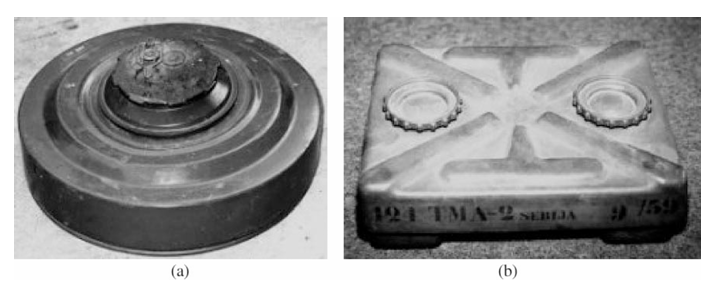
\includegraphics[width=0.7\textwidth]{figs/Huirui/atm_examples.png}
    \caption{Two typical AT Landmines: (a) TM-62M and (b) TMA-2 \cite{paik2002image}.}
    \label{fig:atm_examples}
\end{figure}

\begin{table}[h]
    \centering
    \caption{Specifications for Two Different ATMs (TM-62M and TMA-2) \cite{paik2002image}}
    \label{tab:atm_specs}
    \begin{tabular}{lcc}
        \toprule
        \textbf{Model No.} & \textbf{TM-62M} & \textbf{TMA-2} \\
        \midrule
        Dimensions & Height 112 mm, diameter 316 mm & Height 140 mm, width 260 × 200 mm \\
        Weight & 8.47 kg & 7.5 kg \\
        Case & Steel & Plastic \\
        Sensitivity & 200 kg & 120 kg \\
        \bottomrule
    \end{tabular}
\end{table}

\subsubsection{Anti-Personnel Landmines}

APLs are designed to injure or kill individuals on foot. These mines are typically much smaller than ATLs, with diameters ranging from 6 to 15~cm and explosive weights as low as 0.1–0.5~kg. APLs are generally triggered by very low pressures (often less than 10~kg), making them extremely dangerous and difficult to detect.

APLs can be classified into several subtypes:
\begin{itemize}
    \item \textbf{Blasting mines} (e.g., PRB-M35, PMN) are small, pressure-activated devices buried just beneath the ground surface. They often use plastic or rubber casings to minimize detectability.
    \item \textbf{Bounding fragmentation mines} (e.g., VALMARA-69) are launched into the air before detonation, releasing metal fragments across a wide area.
    \item \textbf{Directional fragmentation mines} (e.g., MON-100) are mounted on the surface and project shrapnel in a specific direction, often over long distances.
\end{itemize}

Figure~\ref{fig:apm_examples} presents four common types of APLs, and Table~\ref{tab:apm_specs} summarizes their technical specifications. Note that blasting types tend to be the smallest and most common in post-conflict zones, whereas bounding and directional mines vary in shape, size, and lethality. Importantly, most APLs are constructed from low- or non-metallic materials such as plastic or rubber, making them highly resistant to conventional metal detection \cite{kaya2017buried}.

\begin{figure}[h]
    \centering
    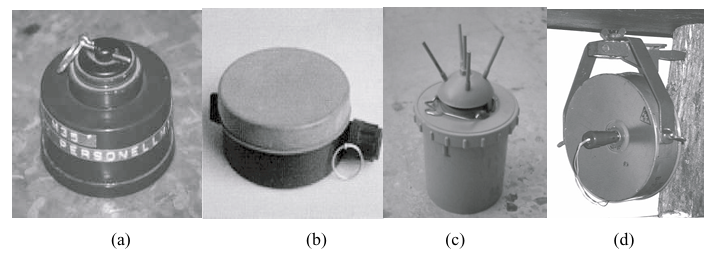
\includegraphics[width=0.9\textwidth]{figs/Huirui/apm_examples.png}
    \caption{Typical APLs: (a) PRB-M35, (b) PMN, (c) VALMARA-69, and (d) MON-100 \cite{paik2002image}.}
    \label{fig:apm_examples}
\end{figure}

\begin{table}[h]
    \centering
    \small
    \caption{Specifications for APLs in Figure~\ref{fig:apm_examples} \cite{paik2002image}}
    \label{tab:apm_specs}
    \begin{tabular}{l p{2.5cm} p{2.5cm} p{3cm} p{3cm}}
        \toprule
        \textbf{Model No.} & \textbf{PRB-M35} & \textbf{PMN} & \textbf{VALMARA-69} & \textbf{MON-100} \\
        \midrule
        Type & Blasting & Blasting & Bounding fragment & Directional fragment \\
        Height & 58 mm & 56 mm & 105 mm & 82 mm \\
        Diameter & 64 mm & 112 mm & 130 mm & 236 mm \\
        Weight & 158 g & 600 g & 3.3 kg & 5.0 kg \\
        Case & Plastic & Rubber & Plastic & Steel \\
        Sensitivity & 8 kg & 8 kg & 10.8 kg (direct), 6 kg (trip wire) & Depends on fuses \\
        Lethal range & N/A & N/A & Radius 27 m & 100 m by 9.5 m arc \\
        \bottomrule
    \end{tabular}
\end{table}

Given their smaller size, lower detonation pressure, and frequent use of low- or non-metallic casings, APLs present a considerably more challenging detection problem than ATLs, making them ideal test cases for evaluating the effectiveness of our airborne sensing systems. From a technical point of view, designing the system to reliably detect smaller APLs ensures that larger and more detectable ATLs can also be identified with relative ease. Furthermore, APLs are responsible for the vast majority of landmine-related civilian injuries and deaths in post-conflict zones \cite{unmas2021handbook}, which amplifies the humanitarian importance of targeting this category. For these reasons, our project focuses on the detection of anti-personnel landmines.
